\section{Datasets, Triggers and MC samples}
%%%%%%%%%%%%%%%%%%%%%%%%%%%%%%%%%%%%%%%%%%%%%%%%%%%%%%%%%%%%%%%%%%%%%%
\label{sec:Datasets}

This analysis relies on the published \hww measurements~\cite{Chatrchyan:2013iaa} in terms of code, selections and background estimates for both the ggH and VBF prodocution mechanisms.

%-------------------------------------------------------------------------------
\subsection{Datasets and triggers\label{subsec:Datasets}}

The datasets used for the analysis correspond to 19.4\ifb at $\sqrt{s}=8$\TeV  of integrated luminosity composed of the following CMS data taking periods during 2012: 2012A (892~$\mathrm{pb}^{-1}$), 2012B (4440~$\mathrm{pb}^{-1}$), and 2012C (6898~$\mathrm{pb}^{-1}$) and 2012D (7238~$\mathrm{pb}^{-1}$).
Data have been checked and validated and only data corresponding to good data taking quality are considered.
The $\mathrm{e}^{\pm}\mu^{\mp}$ final state is considered in this analysis.
%The following five Primary Datasets have been used for the signal extraction: SingleElectron, SingleMu and MuEG (Muon-ElectronGamma).

For the data samples, the events are required to fire one of the unprescaled
single-electron, single-muon or muon-electron triggers.
A full description of these triggers in given in~\cite{AN-2012-228} for 8 \TeV data. Although identification and isolation criteria are
also applied, a brief overview of the HLT \pt criteria on the leptons
is given in Table~\ref{tab:trigger}. While the HLT lepton \pt thresholds of 17 and 8 \GeV for the double
lepton triggers accommodate the offline lepton \pt selection of 20 and 10 \GeV, the higher \pt thresholds
in the single lepton triggers help partially recovering double lepton trigger inefficiencies
as a high \pt lepton is on average expected due to the kinematic of the Higgs decay. 

\begin{table}[h]
\begin{center}
\caption{Highest transverse momentum thresholds applied in the lepton triggers at the HLT level. 
         Double set of thresholds indicates the thresholds for each leg of the double lepton triggers.}
\begin{tabular}{ccc}
\hline
Trigger Path      & 7 \TeV                   & 8 \TeV \\
\hline \hline
Single-Electron   & $\pt > 27 $ \GeV         & $\pt > 27   $ \GeV         \\  
Single-Muon       & $\pt > 15 $ \GeV         & $\pt > 24   $ \GeV         \\ 
%Double-Electron   & $\pt > 17$ and $8 $ \GeV & $\pt > 17$ and $8   $ \GeV         \\ 
%Double-Muon       & $\pt > 17$ and $8 $ \GeV & $\pt > 17$ and $8   $ \GeV         \\ 
Muon-Electron     & $\pt > 17$ and $8 $ \GeV & $\pt > 17$ and $8   $ \GeV         \\ 
Electron-Muon     & $\pt > 17$ and $8 $ \GeV & $\pt > 17$ and $8   $ \GeV         \\ 
\hline
\end{tabular}
\label{tab:trigger} 
\end{center}
\end{table}

No trigger requirement is made on the simulated events but the combined trigger efficiency
is estimated from data and applied as a weight to all simulated events. The detailed trigger efficiencies 
and the weighting procedure can be found in Appendix C of~\cite{AN-2013-022}~\cite{AN-2013-052}. The average
trigger efficiency for signal events that pass the full event selection
is measured to be about 96\% in the $e\mu$ final state for a Higgs 
boson mass of about 125\GeV. 

%-------------------------------------------------------------------------------
\subsection{Monte-Carlo samples\label{subsec:MC}}

Several Monte Carlo event generators are used to simulate the signal and background processes:
\begin{itemize}
\item The first version of the \textsc{Powheg} program~\cite{Kramer:2005hw,Frixione:2007vw,Lavesson:2008ah,Alioli:2008tz, Nason:2009ai} (\textsc{Powheg V1}) provides event samples for the \hww signal
for the gluon fusion (ggH) and VBF production mechanisms, as well as \ttbar and tW processes~\cite{Alioli:2011as}, with NLO accuracy.
\item The $\mathrm{qq} \to \mathrm{W^{+}W^{-}}$, Drell-Yan, ZZ, WZ, W$\gamma$, W$\gamma^*$, tri-bosons and W+jets processes are generated using
the \textsc{Madgraph 5.1.3}~\cite{Alwall:2014hca} event generator.
\item The gg$\to \mathrm{W^{+}W^{-}}$ process is generated using the \textsc{gg2ww} 3.1 generator ~\cite{Binoth:2006mf} and its cross section is scaled to the approximate NLO prediction~\cite{Bonvini:2013jha,Passarino:2013bha}.
\item The VH process is simulated using \textsc{pythia 6.426}~\cite{Sjostrand:2006za}.
\end{itemize}
For leading-order generators samples, the \textsc{cteq6l}~\cite{Lai:2010nw} set of parton distribution functions
(PDF) is used, while \textsc{ct10}~\cite{Lai:2010vv} is used for next-to-leading order (NLO) ones.
Cross section calculations~\cite{Dittmaier:2011ti} at next-to-next-to-leading order (NNLO) are used for the \hww process, while NLO calculations are used for background cross sections.
The $\hww$ process simulation is reweighted so that the \pth{} spectrum and inclusive production cross section closely match the SM calculations that have NNLO+NNLL pQCD accuracy in the description of the Higgs boson inclusive production, in accordance with the LHC Higgs Cross Section Working Group recommendations~\cite{Heinemeyer:2013tqa}.
The reweighting of the \pth{} spectrum is achieved by tuning the \textsc{Powheg} generator, as described in detail in Ref.~\cite{Alioli:2010xd}.
Cross sections computed with NLO pQCD accuracy~\cite{Heinemeyer:2013tqa} are used for the background processes.
The contribution of the \ttH production mechanisms is checked to be negligible in each bin of \pth (below 1\%) and is not included among the different production mechanisms. In Fig.~\ref{fig:signal_comp} the relative fraction of the four production mechanisms is shown for each \pth bin.

\begin{figure}[htb]
\centering
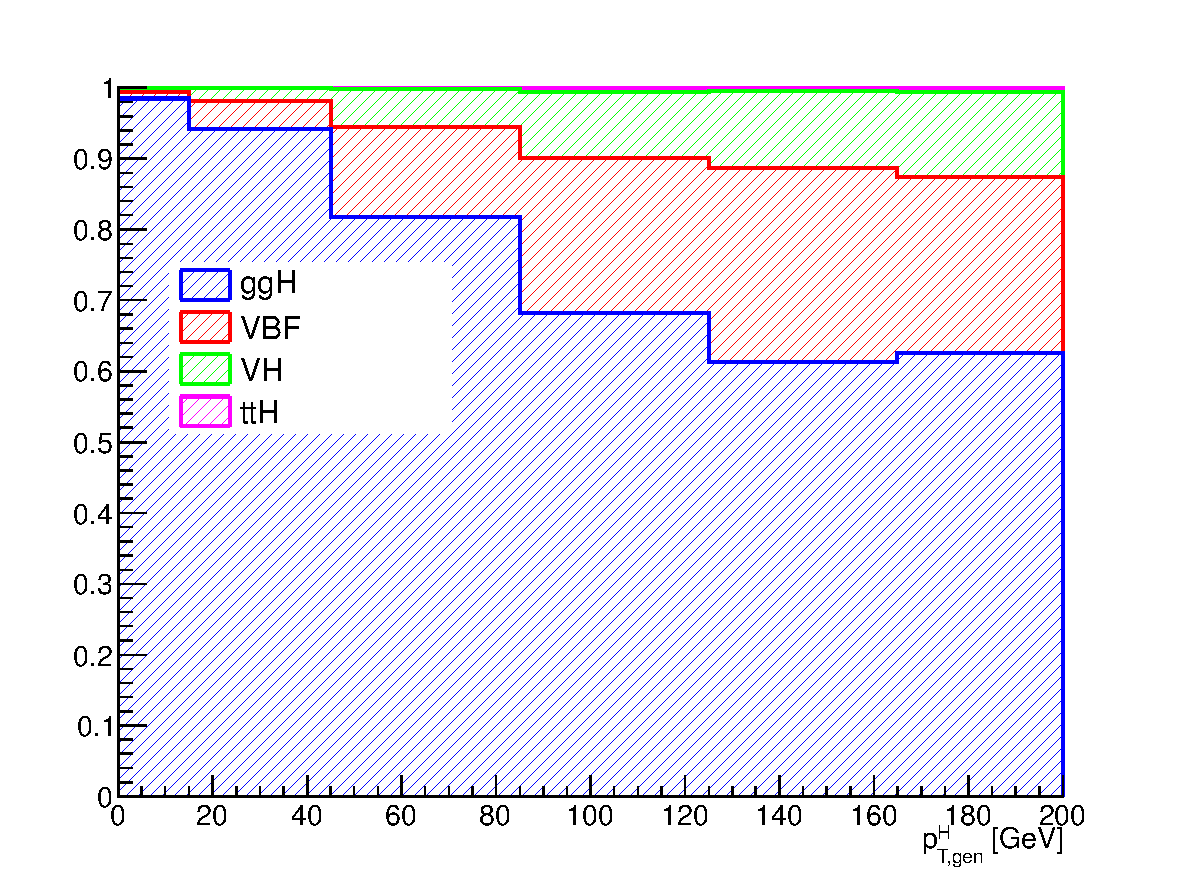
\includegraphics[width=0.7\textwidth]{images/signal_composition_ttH.pdf}
\caption{Relatve fraction of ggH, VBF, VH and ttH in each bin of the Higgs boson transverse momentum.}\label{fig:signal_comp}
\end{figure}


For all processes, the detector response is simulated using a detailed description of the CMS detector, based on the \textsc{Geant4} package~\cite{Agostinelli:2002hh}.

Minimum bias events are superimposed on the simulated events to emulate the additional 
pp interactions per bunch crossing (pileup). The number of pile-up events simulated in the MC samples
(in the same bunch crossing, in time, or in the previous or following one, out of time pileup)
have been generated poissonianly sampling from a distribution similar to what
is expected from data. For a given range of analyzed runs, the mean number of pileup interactions per bunch crossing is estimated per luminosity block using the instantaneous luminosity provided by the LHC, integrated over the entire run range and normalized.
The average number of pileup events per beam crossing in the 2011 data is about 10, and in the 2012 data it is about 20.

The simulated events are reweighted to correct for observed differences between data and simulation in the number of pileup events, as shown in Fig.~\ref{fig:nvertices}, trigger efficiency, and lepton reconstruction and identification efficiencies~\cite{Chatrchyan:2013iaa}.

\begin{figure}[htb]
\centering
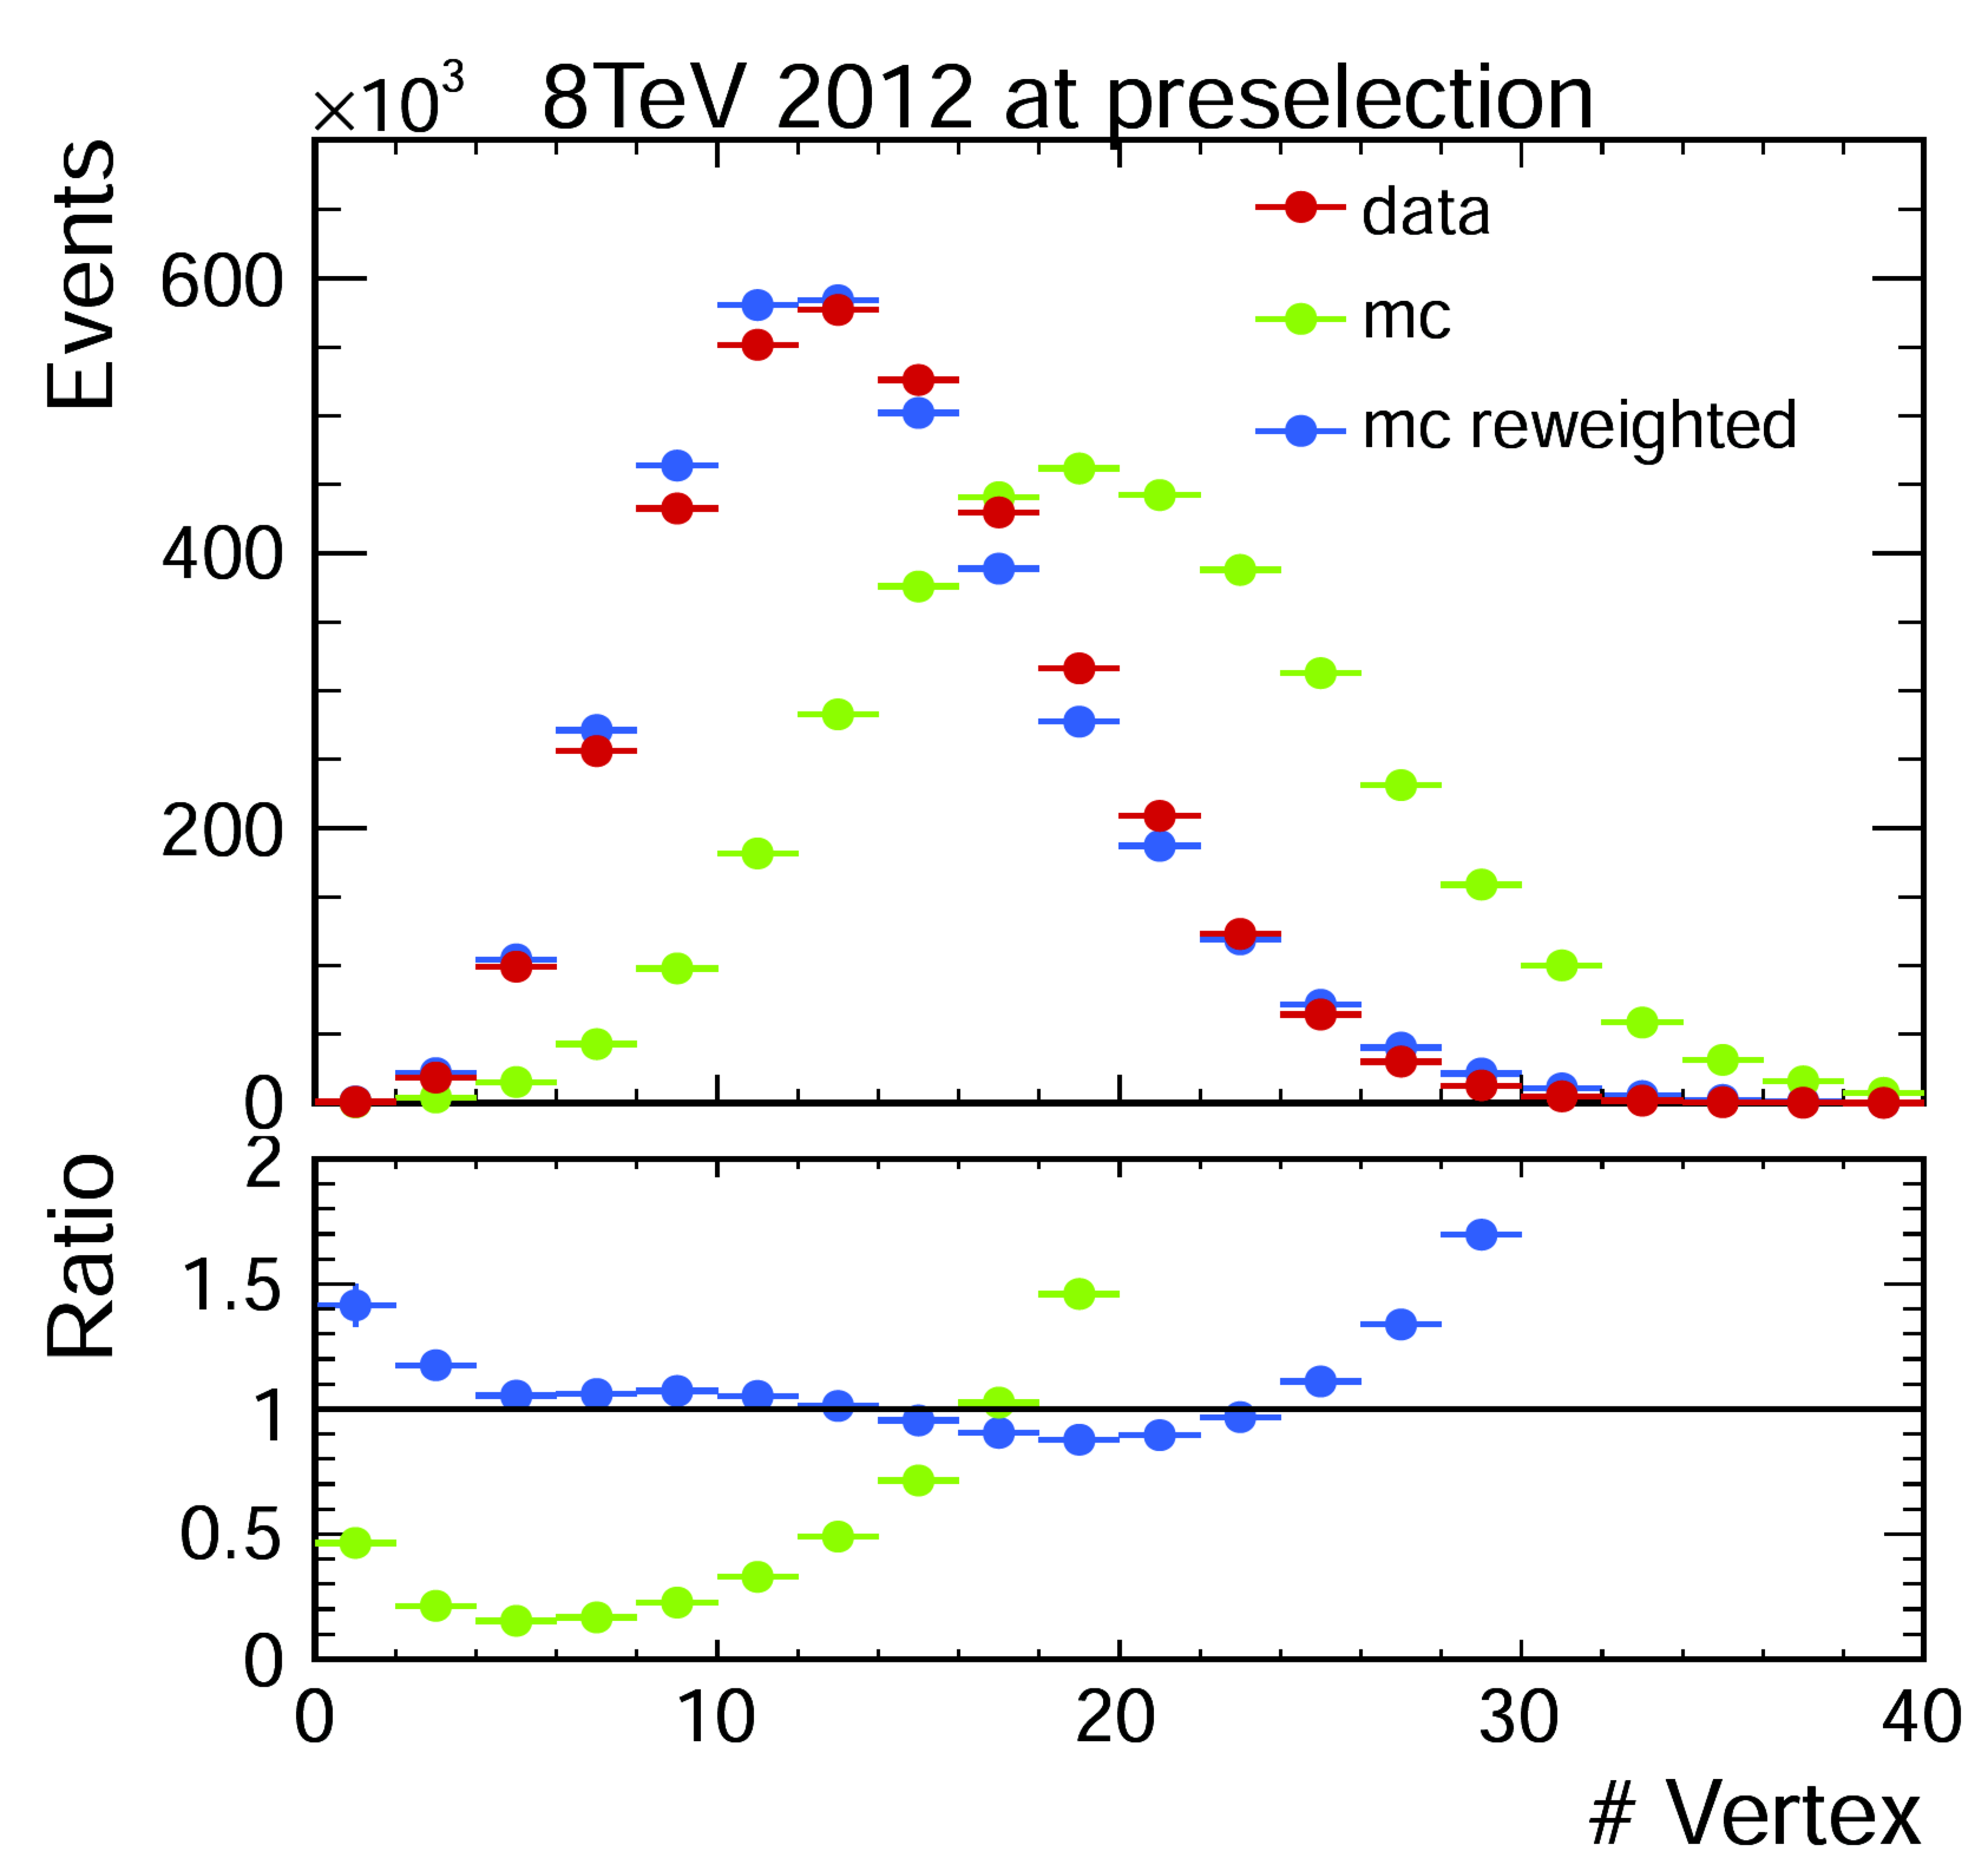
\includegraphics[width=0.7\textwidth]{images/nvertex.pdf}
\caption{Distribution of the number of vertices in data and in simulation, before and after applying the pile-up reweighting.}\label{fig:nvertex}
\end{figure}

For the comparison of the measured unfolded spectrum with the theoretical predictions, two additional MC generators are used for simulating the SM Higgs boson production in the ggH process: \textsc{HRes} 2.3~\cite{deFlorian:2012mx,Grazzini:2013mca} and the second version of the \textsc{Powheg} generator (\textsc{Powheg V2})~\cite{Bagnaschi:2011tu}.
\textsc{HRes} is a partonic level MC generator that computes the SM Higgs
boson cross section at NNLO accuracy in pQCD and performs the NNLL
resummation of soft-gluon effects at small \pt. The central predictions of
\textsc{HRes} are obtained including the exact top and bottom quark mass contribution to
the gluon fusion loop, fixing the renormalization and factorization scale central values at a Higgs boson mass of 125\GeV. The cross section normalization is scaled, to take into account electroweak corrections, by a factor of 1.05 and the effects of threshold resummation by a factor of 1.06~\cite{Actis:2008ug,Catani:2003zt}. The upper and lower bounds of the uncertainties are obtained by scaling up and down both the renormalization and the factorization scales by a factor of two.
The \textsc{Powheg V2} generator is a matrix element based generator that provides a NLO description of the ggH process in association with zero jets, taking into account the finite mass of the bottom and top quarks.
The \textsc{Powheg} prediction is tuned using the \textsc{Powheg} damping factor \textit{hdump} of 104.17~\GeV, in order to match the \pth{} spectrum predicted by \textsc{HRes} in the full phase space. This factor reduces the emission of additional jets in the high \pt regime, and enhances the contribution from the Sudakov form factor in the limit of low \pt.
The \textsc{Powheg} generator is interfaced to the \textsc{JHUGen} generator version 5.2.5~\cite{Gao:2010qx,Bolognesi:2012mm,Anderson:2013afp} for the decay of the Higgs boson to a W boson pair and interfaced with \textsc{Pythia 8}~\cite{Sjostrand:2007gs} for the simulation of parton shower and hadronization effects.
